\section{Dataset and Method} \label{sec:dataset_and_method}

\subsection{Mathematical Model}\label{subsec:mathematical_model}

\Cref{fig:model_selection_approach} shows the approach toward the selection of a suitable model. With this system, we can handle up to N models. \Cref{eq:v_score} shows the mathematical formula used to calculate the V scores of the models. These V scores will allow the system to select the appropriate model.

\begin{equation}\label{eq:v_score}
    V_{score} = \left(\sum_{x=1}^{5} w_xP_x\right) - w_6^2P6
\end{equation}

\begin{figure*}
    \centering
    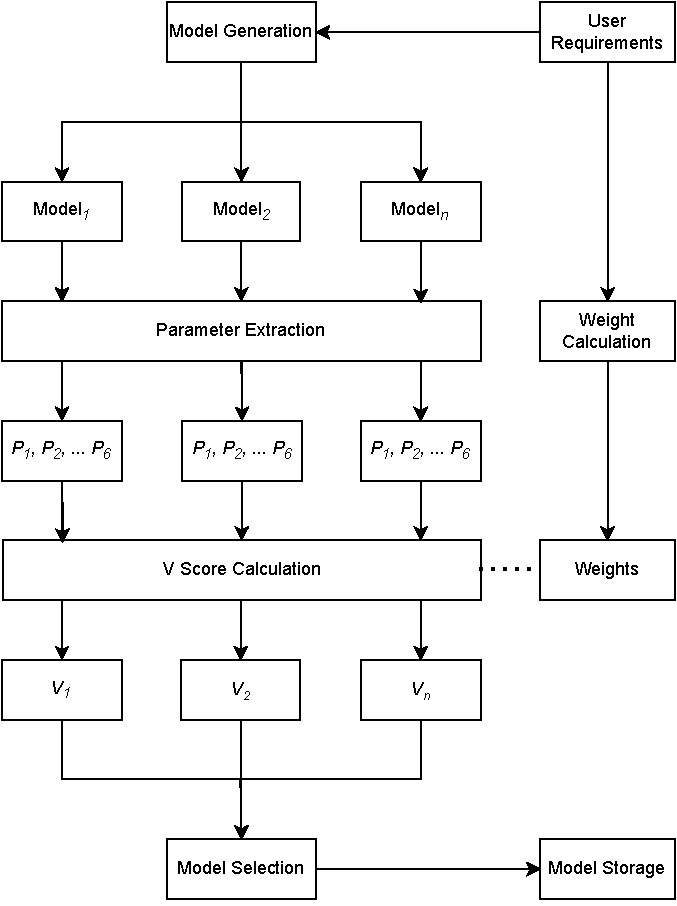
\includegraphics[width=1.4\columnwidth]{media/ch_dataset_and_methods/math_model_relaxed.pdf}
    \caption{Model Selection Approach}
    \label{fig:model_selection_approach}
\end{figure*}

{\responsemod

\subsection{Performance Metrics} \label{subsec:performance_metrics}
The following performance metrics are used in the system for evaluation of the models:

\subsubsection{Accuracy Score}\label{subsubsec:accuracy_score}
The accuracy score is a fraction of the correct prediction by model with respect to total
predictions by model. It can be represented by following formula:
\begin{equation*}\label{eq:accuracy_score}
    Accuracy = \frac{TP+TN}{TP+TN+FP+FN}
\end{equation*}

\subsubsection{Precision score}\label{subsubsec:precision_score}
The precision score is a fraction of the correct positive predictions with respect to all
positive predictions of the model. Higher precision scores result in fewer false positive
predictions. It can be represented by following formula:
\begin{equation*}\label{eq:precision_score}
    Precision = \frac{TP}{TP+FP}
\end{equation*}

\subsubsection{Recall score}\label{subsubsec:recall_score}
The recall score is the fraction of correct positive predictions with respect to all
predictions of the class. It can be represented by following formula:
\begin{equation*}\label{eq:recall_score}
    Recall = \frac{TP}{TP+FN}
\end{equation*}

\subsubsection{F1 Score}\label{subsubsec:f1_score}
The F1 score is the weighted average of the recall score and precision score of the model. F1 scores are more reliable than accuracy scores in case of biased or uneven dataset. It can be represented by following formula:
\begin{equation*}\label{eq:f1_score}
    F1 = 2 \cdot \frac{Recall \cdot Precision}{Recall + Precision}
\end{equation*}
or
\begin{equation*}\label{eq:f1_score_2}
    F1 = \frac{TP}{TP+\frac{1}{2}(FP+FN)}
\end{equation*}

\subsubsection{ROC Score}\label{subsubsec:roc_score}
The ROC is a classifier's predictive quality that compares and visualizes the trade-off between the model's sensitivity and specificity. In graphical format, the area under it gives a relationship between false positives and true positives. The higher these areas are, the better the predictive quality of the model.

\subsubsection{Prediction Time}\label{subsubsec:prediction_time}
Prediction times are nothing but the amount of time required by the classifier to make predictions for certain testing datasets. A model with a lower prediction time is desirable.

\subsection{Methodology} \label{subsec:methodology}
The system accepts the data and parameter preferences from the user. The parameter preferences are used to generate weightage. This weightage is stored in memory for future use. The dataset from the user is split into an 80-20 ratio to generate a training and evaluation dataset. These datasets are stored on a drive for future use.

The training dataset is loaded into the system simultaneously. The model generated is used to generate the pre made models. These models are trained with a training dataset and stored on disk for the evaluation process.

In the evaluation process, the evaluation dataset is used on the trained models along with weightage generated from user parameter preferences. The evaluation process produces the Vscore. The model with the highest Vscore is selected as the most suited model.
}

\subsection{Dataset}
The ECG readings in this paper are obtained from the MIT-BIH arrhythmia database [\citenum{dataset_heartbeat}]. This database is used for automated training and evaluation. This dataset was published in 1999 by MIT-BIH as an open-source database; it consists of training and testing datasets. This database is further divided into four equal parts for analysis. Each training set contains 21888 signals, and the testing set contains 5473 signals.